\chapter{Exploratory Experiments in a Rainforest Environment}\label{chap:technical}
	In this chapter, we explain our motivating scenario in more detail, explore the sensor hardware and software that we researched and outline the results of experiments we undertook in the Malaysian rainforest. As highlighted in Section \ref{int:mot}, we have been working with Cardiff University School of Biosciences to design and deploy a WSN that utilises local and global knowledge, using an area of rainforest in Malaysia owned by the Sabah Wildlife Department, called Danau Girang.

The structure of this chapter is as follows. Section \ref{tech:motiv} explains what we aimed to deploy in Danau Girang and what our considerations were. Section \ref{tech:hw} introduces sensor hardware that is in use today and details the choices we made. Section \ref{tech:wireless} details the transmission medium choices we tried and also shows the results of experiments performed in both the UK and Malaysia. Section \ref{tech:sw} explains some of the software applications we developed in order to process sensed data on the nodes. Finally, Section \ref{tech:conc} summarises our findings and explains the choices we made for the sensor nodes we used in Danau Girang Field Centre (DGFC). 

\section{Danau Girang Field Centre}\label{tech:motiv}
Based in Sabah, Malaysia, Danau Girang Field Centre is located in Lot 6 of the Lower Kinabatangan Wildlife Sanctuary (LKWS), surrounded by secondary rainforest that had been logged up until the 1970s. Experiencing a wet season from October to February and a dry season from March to September, the LKWS can receive more than 500mm of rainfall during the rainy season, dropping to lows of around 150mm during the dry seasons \cite{Walsh2009}, and up to 100\% humidity all year round. 

		\begin{figure}[h]
		\centering
		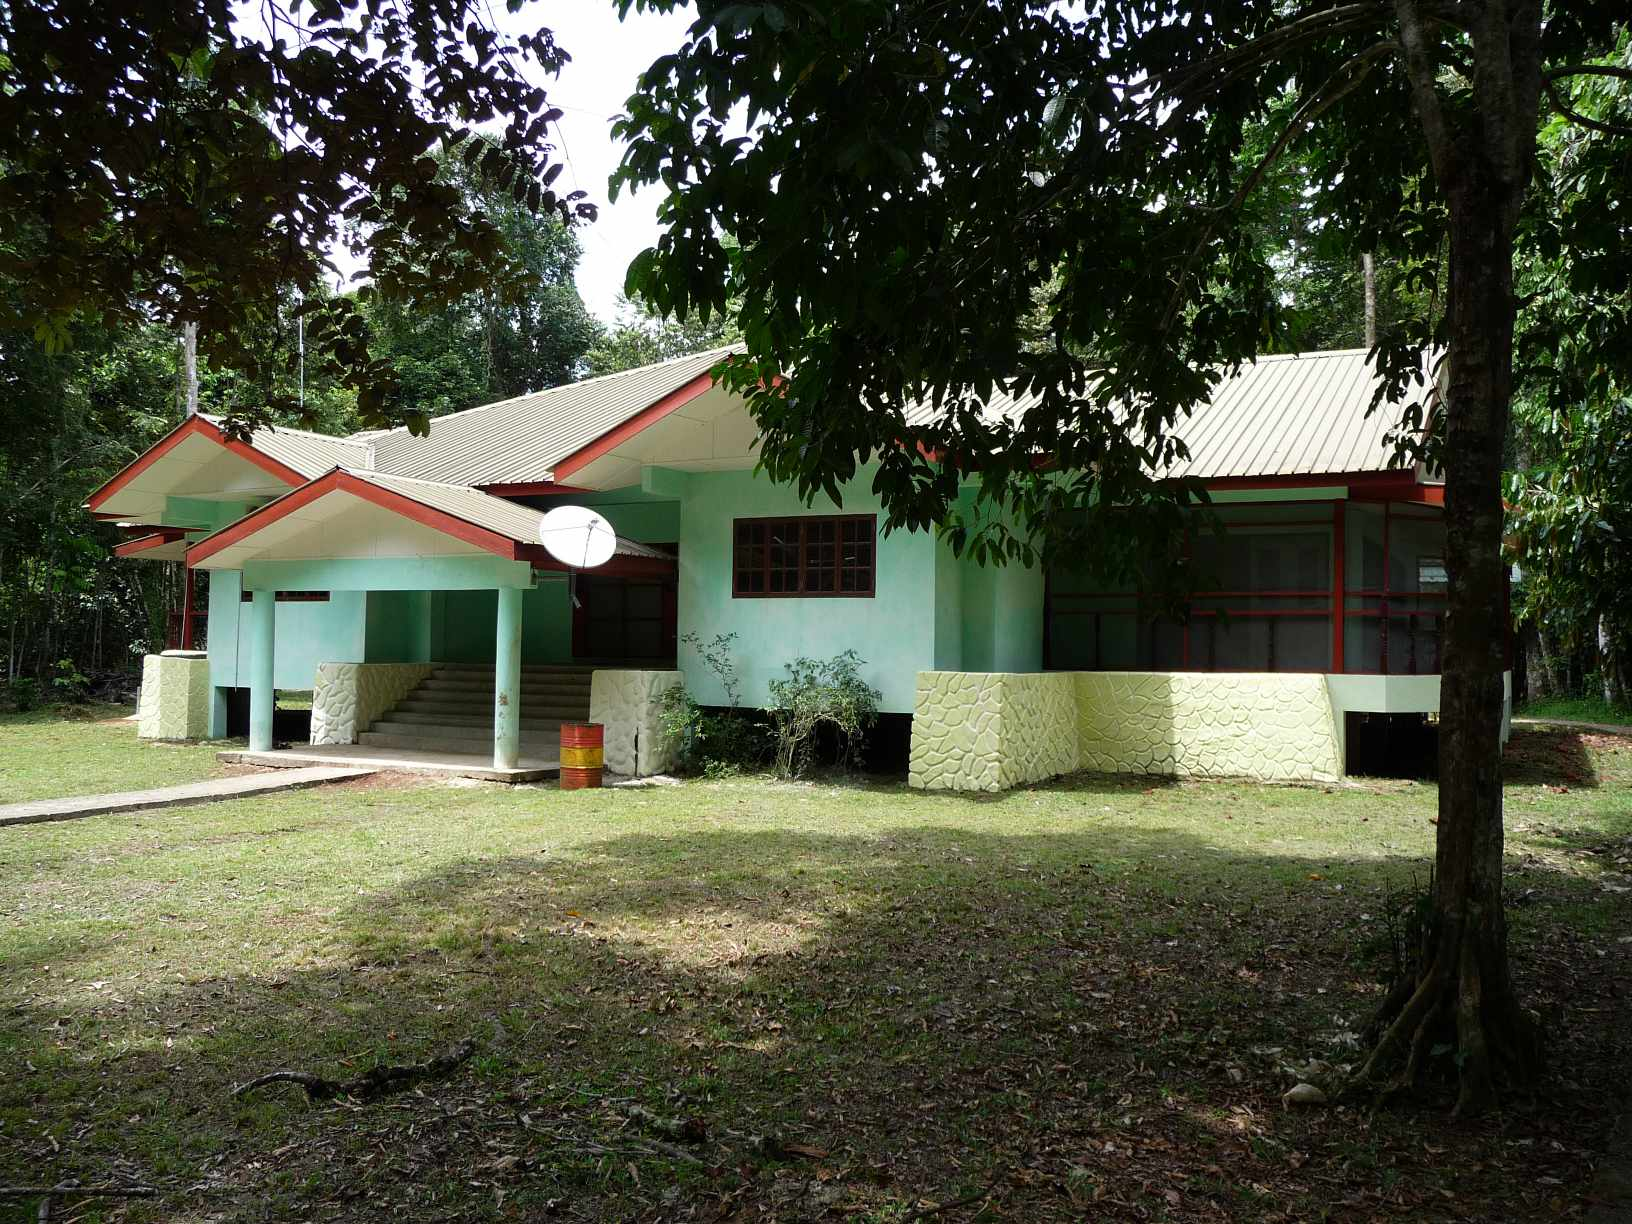
\includegraphics[width=\textwidth]{Chap3/figures/field_centre.JPG}
		\caption{The Main Buidling at DGFC}
		\label{tech:fig:main}
		\end{figure}

Danau Girang is in a unique location, situated in a rainforest corridor (figure \ref{tech:fig:map}) that joins two areas of rainforest together, with the corridor surrounded by palm oil on each side. Because of this, animals use the corridor to move between the rainforest regions and some use it to enter the palm oil plantation for new feeding grounds. This gives the DGFC insight into the movement patterns of these animals in the corridor as well as in the rainforest itself, with a wide variety of species that are not commonly seen in other tropical regions of the world. Due to the remote nature of the centre, power is provided by a set of diesel generators which, typically, provide power from 10 am to 1 pm and 5pm to 11pm daily. Wireless Internet access is provided by satellite with speeds approximating 56kbps, although the upload speeds are considerably faster than downloads.

		\begin{figure}[h]
		\centering
		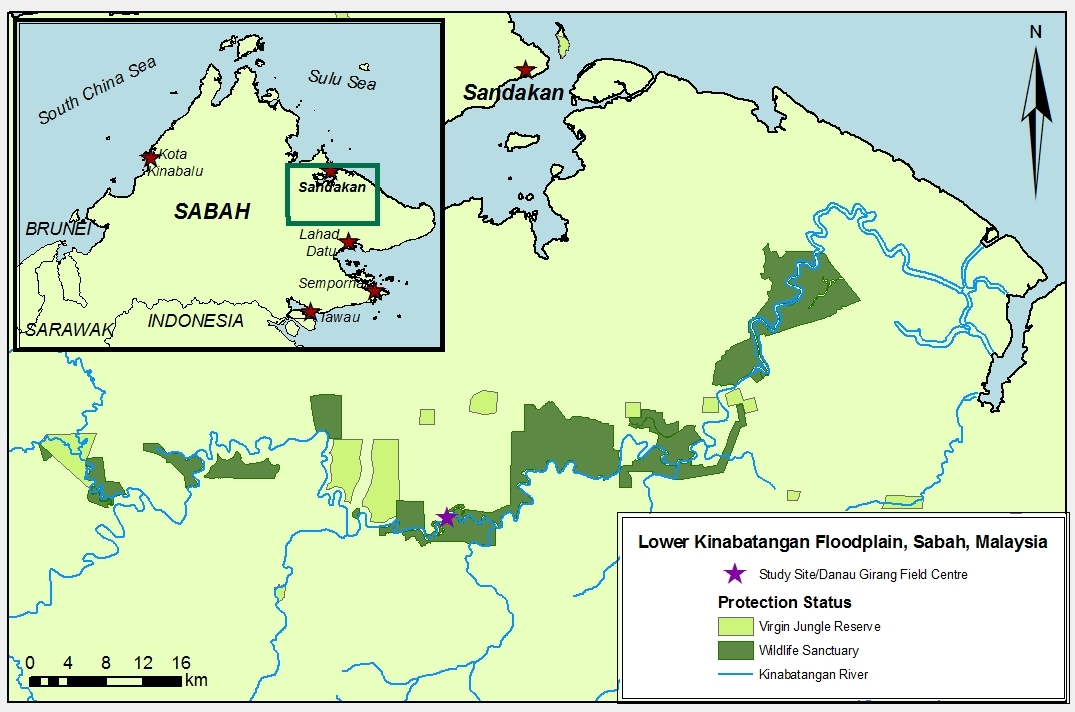
\includegraphics[width=\textwidth]{Chap3/figures/dgfc_map}
		\caption{Map of Danau Girang in relation to Sabah Malaysia}
		\label{tech:fig:map}
		\end{figure}

The corridor monitoring programme is a scheme that has been in place for more than five years, using wildlife cameras to track the movement of animals through the rainforest corridor and to capture species that are rare or unique to South-East Asia, such as the Bornean clouded leopard. Currently, Reconyx Hyperfire HC500 (Figure \ref{tech:fig:cam}) cameras are being used \cite{Reconyx}. These are standalone cameras that capture a user-defined number of images which are saved to an SD card. A trigger is caused by an infrared (IR) motion sensor when an object causes the IR beam to break. 
	
	\begin{figure}[h]
		\centering
		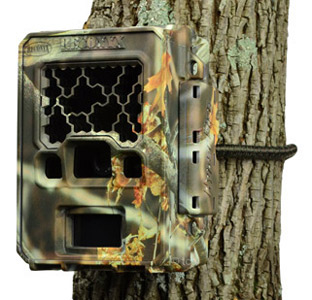
\includegraphics[width=0.7\textwidth]{Chap3/figures/hc500}
		\caption{Reconyx HC500 Camera}
		\label{tech:fig:cam}
		\end{figure}

Images must be manually collected every two weeks from the cameras and the batteries are changed at that point as well, although a typical charge should last three months. In the field, the batteries last a matter of weeks shortly after the cameras are deployed, this is most likely because, although the cameras are equipped with watertight casing, they are still exposed to moisture when the case is opened every two weeks and 100\% humidity seems to have an impact as well. Silica gel is used to prevent moisture inside the camera. We believe that humidity also reduces the battery life, as the charge drops from three months to around three weeks within the first few months of usage. However, the lack of constant power availability could also affect the charge of the batteries. Because power is not available all day, the batteries are charged for a period of a few hours at a time. Not only does this reduce the number of charge cycles that these batteries can experience but it also means that they are never fully charged within one time period of power availability. Solar recharging is being researched to counteract this. Each camera is secured to a tree and, when placed in higher risk locations, such as known elephant paths, have protective cases as well. 

In 2010, twenty cameras were deployed for six month periods and then relocated based on the needs of the projects at that time. Currently, there are now ninety cameras with a view to expand and dozens of projects within the field centre use the images gathered from these cameras. Initially, it was the job of visiting research students to collect the images but, since the number of deployed cameras has grown, full-time staff have been taken on to maintain them.

Images that have been collected are stored on an external hard drive in the field centre and a spreadsheet is updated with information about each image, such as date, time, camera, filename and location. Research students and, later, staff, manually inspected each image and added their species classification to the spreadsheet. Because so many images came through the field centre each week, this was a long process and it was not uncommon for it to be a few weeks before the images were classified. Research students in charge of the cameras were usually on projects lasting 6 months so, until staff members were recently employed, their methods of cataloguing were quite different. Sometimes, each student created a different spreadsheet for their time at DGFC and ignored the classification of images that did not contain the animal their project was focussed on. While this has improved now, staff members are tasked with combining these spreadsheets from the past few years and classifying all the images that have been left empty.

With image processing, we can automate the classification process. Using common tools and widely accepted methods, such as OpenCV \cite{opencv_library} and object detection libraries \cite{cvblob}, we can use previously classified images as templates. This allows us to determine if a new image contains an object of interest and extract templates of that object to match to new images and classify them to the species level, once a human has classified the original template. Humans can then check the classification and provide feedback on its validity. This removes the wait of weeks for a classification and automates the cataloguing, classification and storing of the images, when received at the field centre. This method should also allow us to alert researchers when our system believes an image of particular interest, such as a rare animal, has been taken. Without humans to classify images down to the species level, we can still use image processing to determine if an image is interesting or empty.

Our belief is that we can use the Lower Kinabtangan wildlife sanctuary (LKWS), and the locations of the existing cameras, to deploy a WSN that uses local knowledge gained from the researchers at DGFC to automate the collection of images, improve the battery life by not exposing the internals of the camera to the elements so often and, most important, prioritise the flow of data through the network by in-network processing. 
	
Three annual visits, in 2011, 2012 and 2013, each lasting three weeks, have been made to DGFC to test out hardware, software and wireless choices, in an effort to optimise the network. These visits have also been used to extract local knowledge from the area and researchers, by semi-structured interviews and watching them work.

\section{Hardware}\label{tech:hw}
	Before any visits were made to DGFC, meetings with staff members of the field centre were held in order to gain a better understanding of the environment and the project. This is where we were alerted to the humidity of the region and the fact that the failure rate of the Reconyx cameras has been as high as 30\%.

Reconyx cameras have no external interface support and the only way to access the images is through the removable SD card. Because of this, there is no way of attaching external sensor hardware to the existing cameras. In-network processing is an important requirement for our WSN and this did limit our choices to nodes that are computationally capable, e.g. the Pandaboard \cite{instruments2012pandaboard}, than more common sensors, e.g. the IMote 2 \cite{Nachman2008}.

In this section, we detail our research into suitable sensor hardware that met the following requirements:
\begin{enumerate}
	\item Able to perform processing of images and metadata
	\item Common interface availability (Serial, USB)
	\item Wireless enabled
	\item Battery-powered
	\item Expandable memory
\end{enumerate}
It should be noted that there are many devices out there that met the above criteria but we selected devices that had a large development community. At the time of writing, there are now many more, but this research was carried out in 2010, when the market for low-cost, high-power, small form factor single board computers (SBCs) was starting to grow. While we did research on many more devices, the three listed below are the devices we physically trialled and tested.
This section also details the modifications we made to any devices we tested in order to ensure they would survive in a humid environment.

\begin{figure}[ht!]
\centering
\begin{subfigure}{.5\textwidth}
		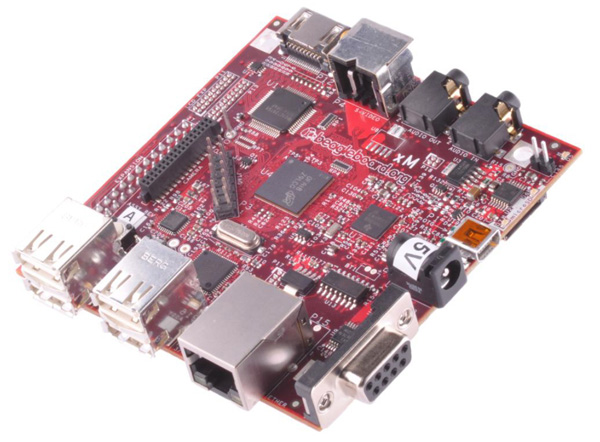
\includegraphics[width=\textwidth]{Chap3/figures/pandaboard}
		\caption{Pandaboard}
		\label{tech:fig:pandaboard}
		\end{subfigure}
\begin{subfigure}{.5\textwidth}
		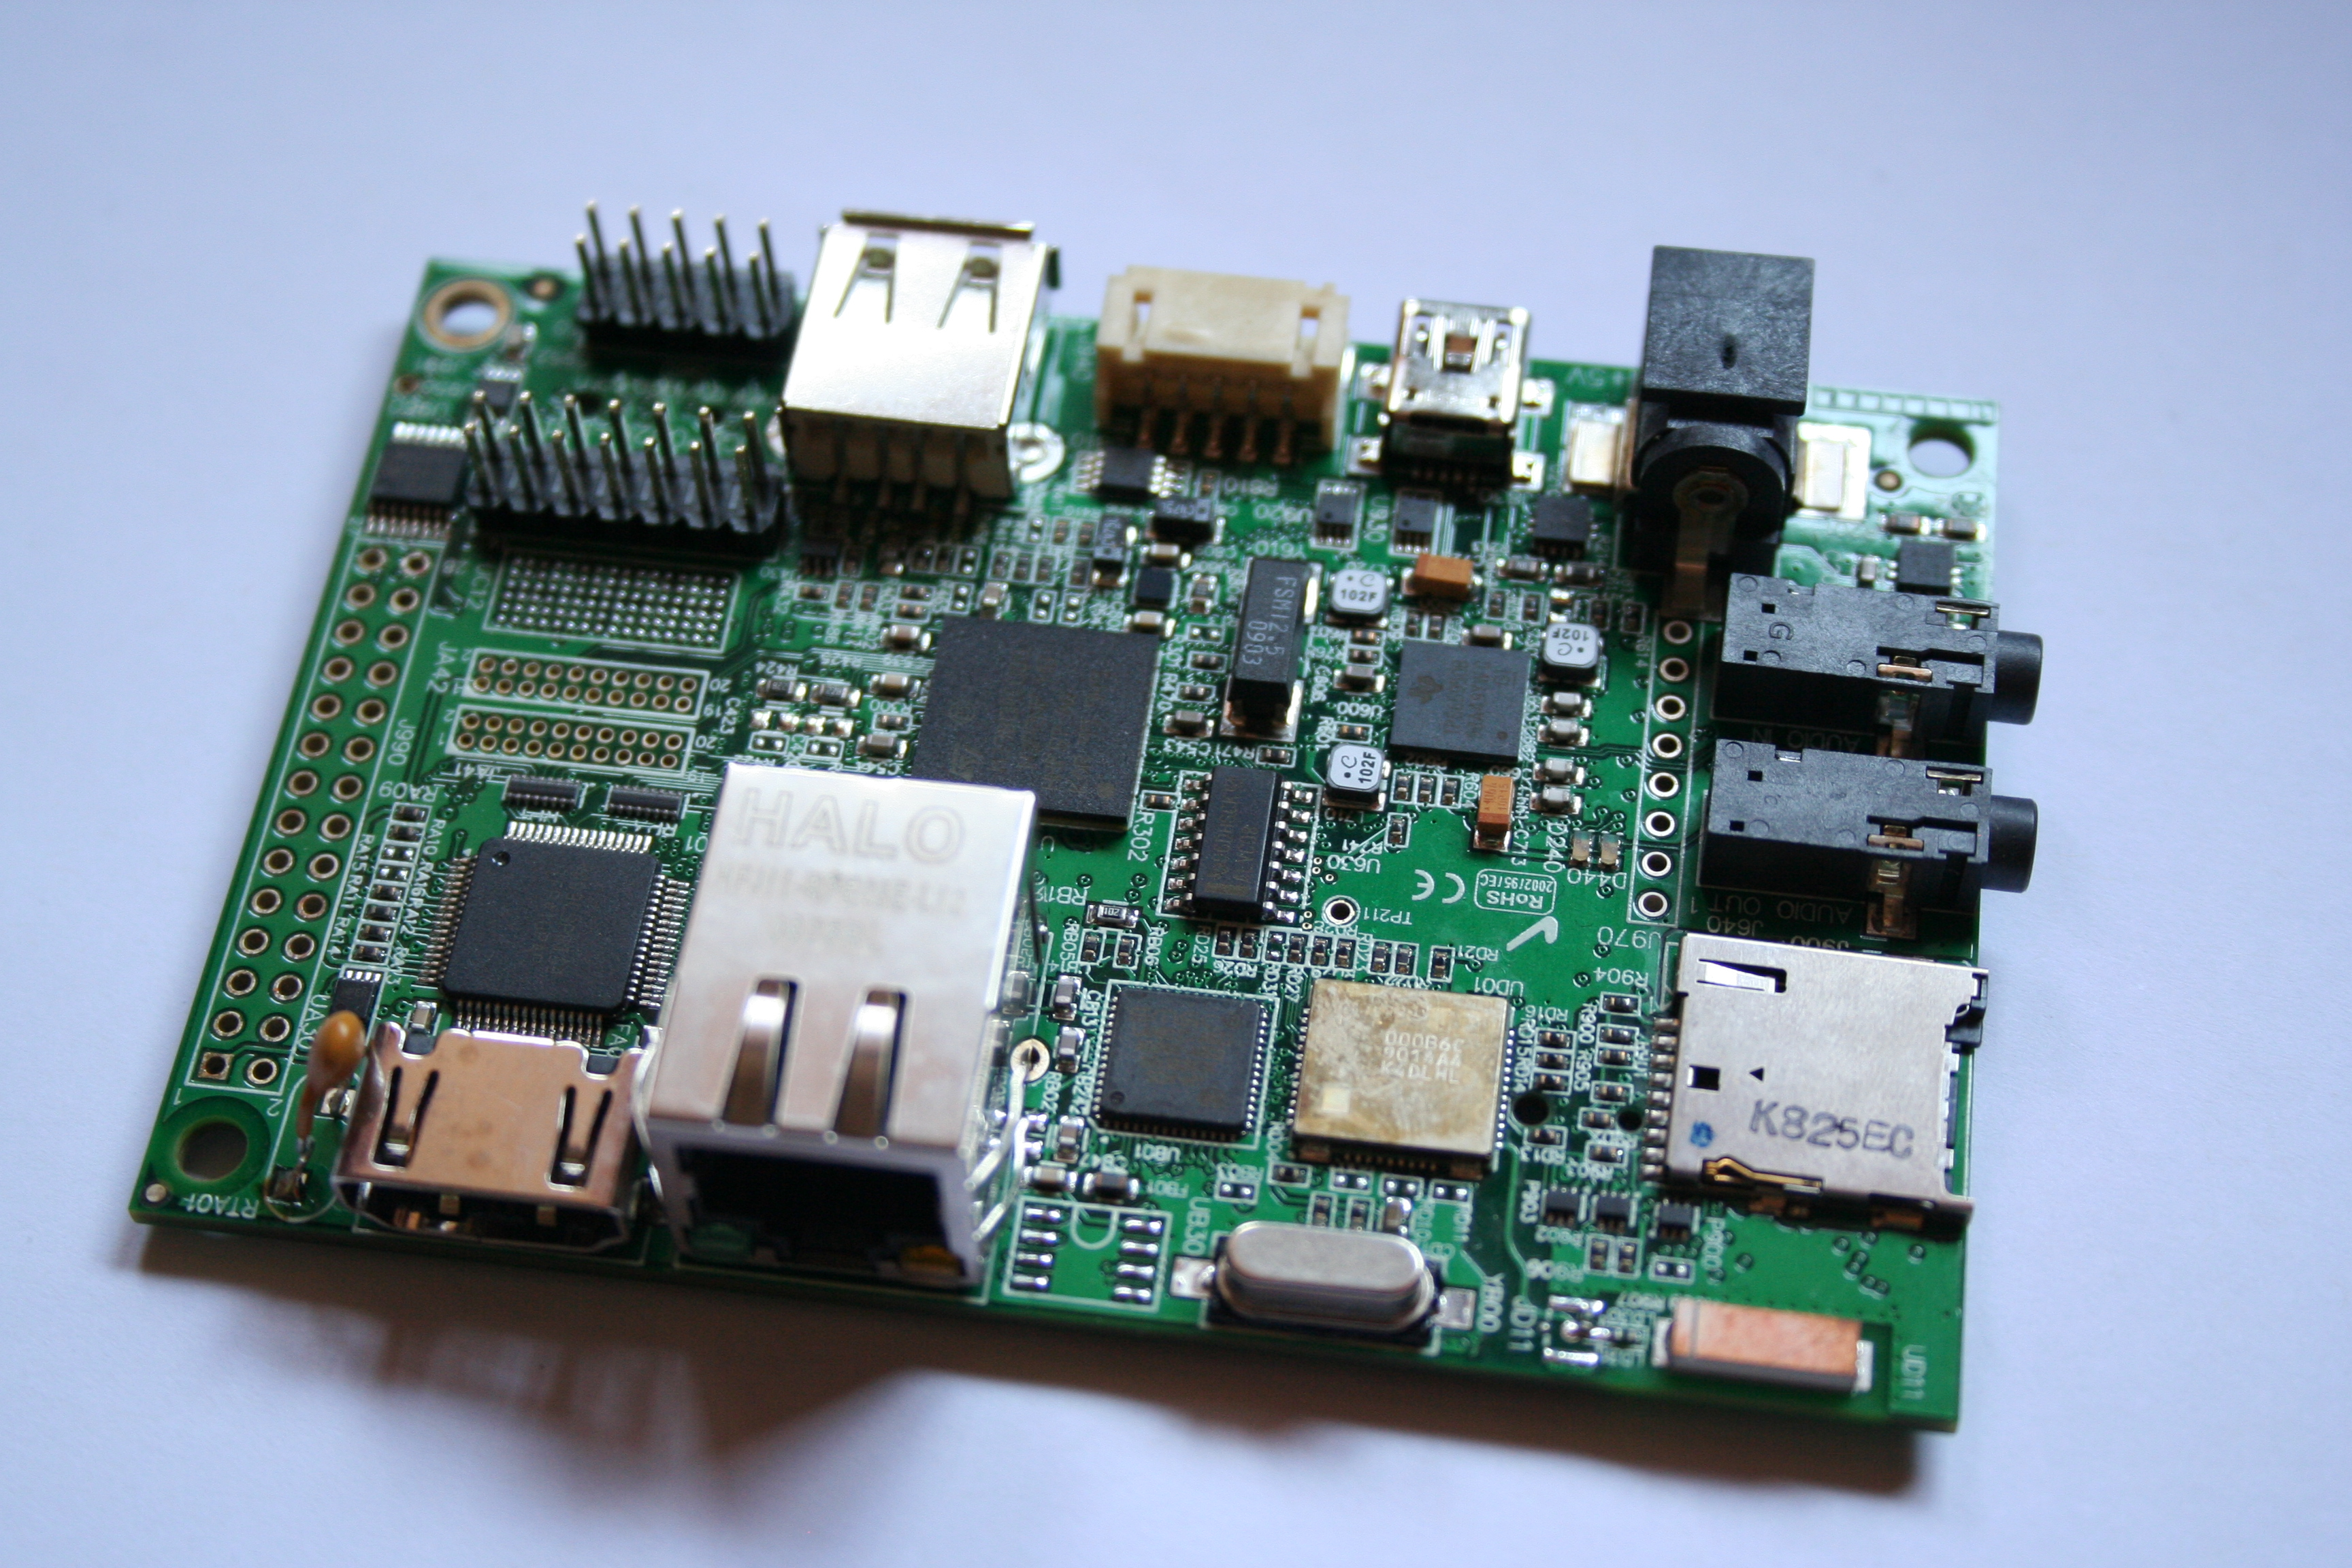
\includegraphics[width=\textwidth]{Chap3/figures/igep}
		\caption{IGEP v2}
		\label{tech:fig:igep}
		\end{subfigure}
\begin{subfigure}{.5\textwidth}
		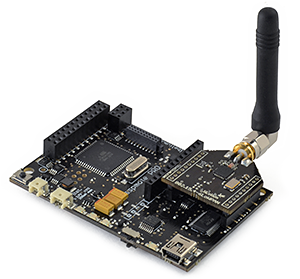
\includegraphics[width=\textwidth]{Chap3/figures/waspmote}
		\caption{Waspmote}
		\label{tech:fig:waspmote}
		\end{subfigure}
\caption{Sensor Node Hardware}
\label{tech:fig:nodes}
\end{figure}

\subsection{Pandaboard}

Texas Instruments supported the development of a reference Single Board Computer (SBC) that had specifications similar to that of a modern smartphone (Figure \ref{tech:fig:pandaboard}) and was capable of running desktop Linux, known as the Pandaboard \cite{instruments2012pandaboard}. A dual core 1GhZ ARM processor with 1GB of RAM, support for external storage, expansion ports, USB, Wi-Fi and Bluetooth in a board the size of two credit cards can be a powerful addition to a data heavy WSN, especially one that deals with images.

There is no mention of Pandaboards in the literature being used in WSNs but the low power of the system and advanced capabilities make it suitable for processing and transmitting data simultaneously. 
	
\subsection{IGEP v2}

The IGEP v2 (Figure \ref{tech:fig:igep}) is another ARM based SBC that uses a 1GhZ single core processor with 512MB RAM and similar connectivity features to the Pandaboard, but around half the size. This does result in a reduced power draw and the device is still capable of running desktop Linux.

Due to the smaller size, and easier commercial availability, the IGEP has been used as a sensor node to record, process and send readings from multiple devices, such as air temperature, GPS and oxygen saturation as part of environmental monitoring \cite{Resch}. In their research, they found that the IGEP achieved 9.1 hours of uptime using a 4000mAH battery, a capacity used in many modern smartphones.

\subsection{Waspmote}\label{tech:waspmote}
The Waspmote (Figure \ref{tech:fig:waspmote}) is a general purpose sensing board that is designed to allow plug-and-play connectivity for multiple sensor modules. The node can be programmed with C++, using the Standard Development Kit (SDK) developed by the manufacturer and uploaded via USB. The processing power is not comparable to the more powerful SBCs, but the 600mAh battery is reported to last three months and the size is much smaller \cite{waspmote}.

One of the primary benefits of the Waspmote is that they are commercially available with an actively maintained programming environment.

\subsection{Discussion} \label{tech:hw:conc}
The capabilities of each of these boards vary greatly from running a subset of C on an embedded OS to running full desktop Linux. Each visit we made to Danai Girang allowed us to test these devices and determine their eligibility for nodes that would survive in the Malaysian rainforest and discover usable radio range data, which we discuss in the next section.

The trade-off with these devices is that the Waspmote nodes, with limiting processing capabilities, is reported to yield a battery life of 6 months. Our tests yielded approximately 3 months, with minimal sleep scheduling, so this number does seem reasonable. However, the IGEP and Pandaboards are able to run any software that has been compiled for an ARM processor and do so within an unrestricted operating system. While this does allow them the flexibility to process data with the same power as a five year old desktop computer, our battery life tests drained the board within 6 hours when using 4 D cell batteries. We managed to increase this number by loading a power-efficient modification of the Arch Linux distro, removing any support for displays or running of a GUI, disabling unused ports and disabling the radios for as much of the uptime as possible. With these changes, we were able to achieve approximately three weeks of running with sleep periods.

Most SBCs, while having a reduced battery life, contain common I/O ports, such as: USB, VGA, Ethernet and Serial. This extensibility enables us to add additional wireless capabilities. For example, sensor nodes may require the use of a long range wireless medium for inter-node communication but the endpoint of a network uses Wi-Fi to allow users to connect to it and upload sensed data to the Internet; this can be done by adding a long-range wireless radio to an I/O port and providing software support.

% Needs to flow better?
\section{Transmission Media}\label{tech:wireless}
	In this section, we explain the experiments we carried out to test the performance of different transmission media in the UK as well as the Malaysian rainforest. While range is the most important feature, a data rate that can handle hundreds of large readings in a day is a requirement, as wildlife cameras can generate ten images each time they are triggered and a high definition image can be up to 1MB in size. Our motivating scenario is focussed on the transmission of sets of 3 images (each around 800KB) for every trigger, where a sensor can trigger hundreds of times in a day.

\subsection{Wi-Fi}\label{tech:wifi}
Wi-Fi was already available on our initial test platforms and the high data rate made it suitable for sending a large volume of images in a short period. We knew that current cameras deployed in DGFC were up to 1km apart and we did not expect to cover that range completely, but we did expect to achieve that coverage by using intermediate nodes.

Research, outlined in Section \ref{bg:trans}, showed that the rainforest could reduce the range by up to 78\% and the ideal maximum range of 2.4GhZ Wi-Fi is 100m \cite{Dhawan2007}. 

We tested Wi-Fi range using two IGEP boards. We selected IGEP boards because they could be powered by 4 D Cell batteries and run a lightweight Linux operating system that allowed us to access information at the network layer, while still running higher level applications. The IGEP nodes we used did not have any additional hardware and the nodes were tested without the use of an external antenna. A Java application was written to periodically scan for available networks and store those results in a text file. One IGEP board was set as the base station and attached to a tree, at the same height it would be if it was attached to a camera, and another was walked to specified points around the base station at defined locations. These locations were chosen to include as many distances as possible and as many different forms of obstacle between the searching node and the base station, such as: line of sight (LOS), medium vegetation or thick trees.
			
This experiment was run in a wooded area in the UK and in the rainforest at DGFC. The specified maximum range of 802.11g is 120m. When considering attenuation and obstacles we were expecting the signal to be reduced by up to 50\% in the UK. However, we found that we received a maximum range of 30m, with LOS. Figure \ref{fig:test} shows the results we experienced, while testing in the UK, some of the drops in signal can be attributed to dense foliage and readings that were not LOS, but a maximum range of 31m, with an SNR of 29.5 dBm, is less than we expected, as the UK does not experience high humidity often.
			
	The graph shows a drop at 22m: this was due to unusually dense foliage that restricted the LOS between the base station and the receiving node. With five runs of this test we observed the same results. The primary aim of this experiment was to show the viability of Wi-Fi and to ensure our application functioned as intended, which it did. Further experiments could have been run to remove the anomaly but the results of the experiments in Danau Girang were the focus.
		 
	Despite the poor range from the tests in the UK, it was consistent with other studies reporting signal degradation of up to 78\% in areas with dense foliage. We visited Danau Girang in 2011 to gather the requirements of the network and ensure the hardware is able to survive the humidity. Range experiments were run in the rainforest to see if a more humid environment impacts range any further, Figure \ref{fig:test} shows this.

\begin{figure}[ht!]
\centering
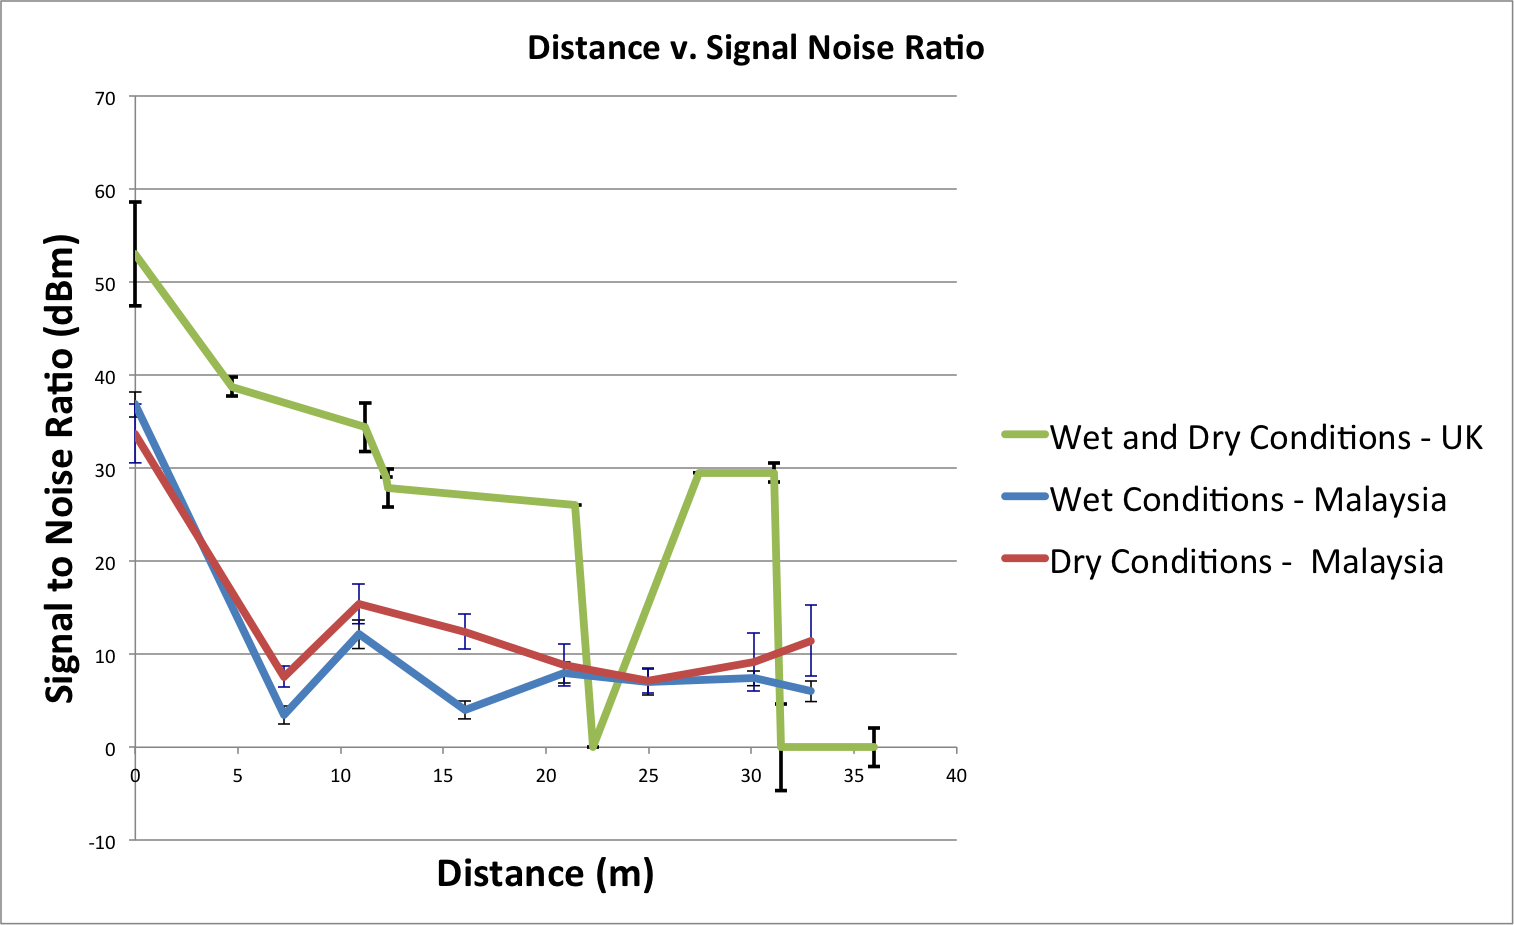
\includegraphics[width=0.7\textwidth]{Chap3/figures/combined_snr.png}
% \begin{subfigure}{0.9\textwidth}
%   \centering
%   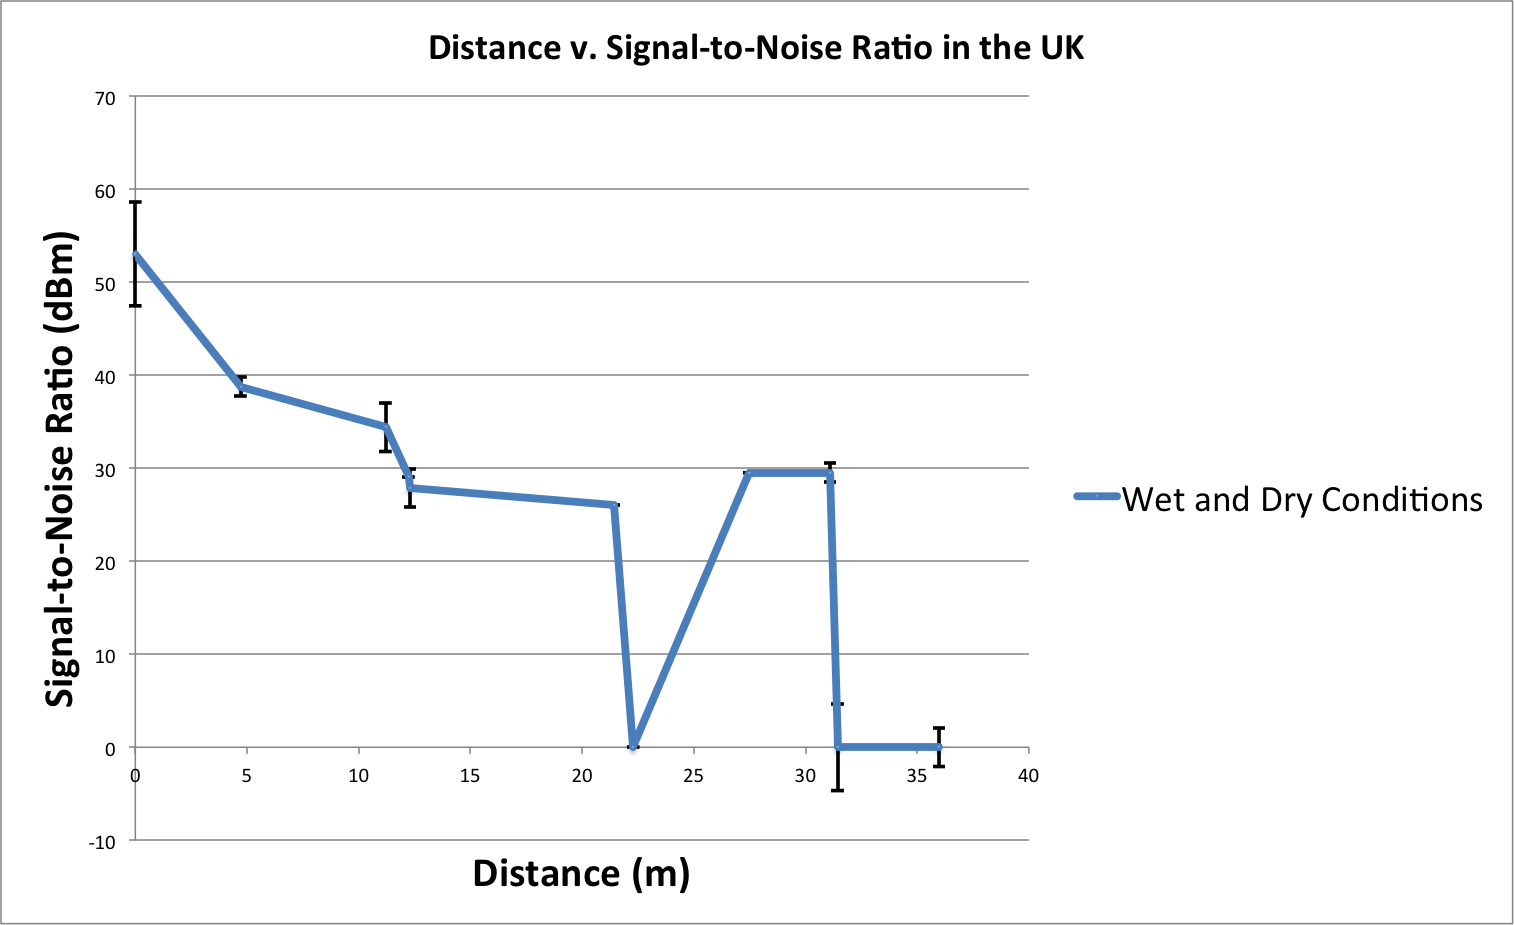
\includegraphics[width=\textwidth]{Chap3/figures/bp_snr.png}
%   \caption{UK Woodland}
% 	\label{cardiffsnr}
% \end{subfigure}
% \begin{subfigure}{0.9\textwidth}
%   \centering
%   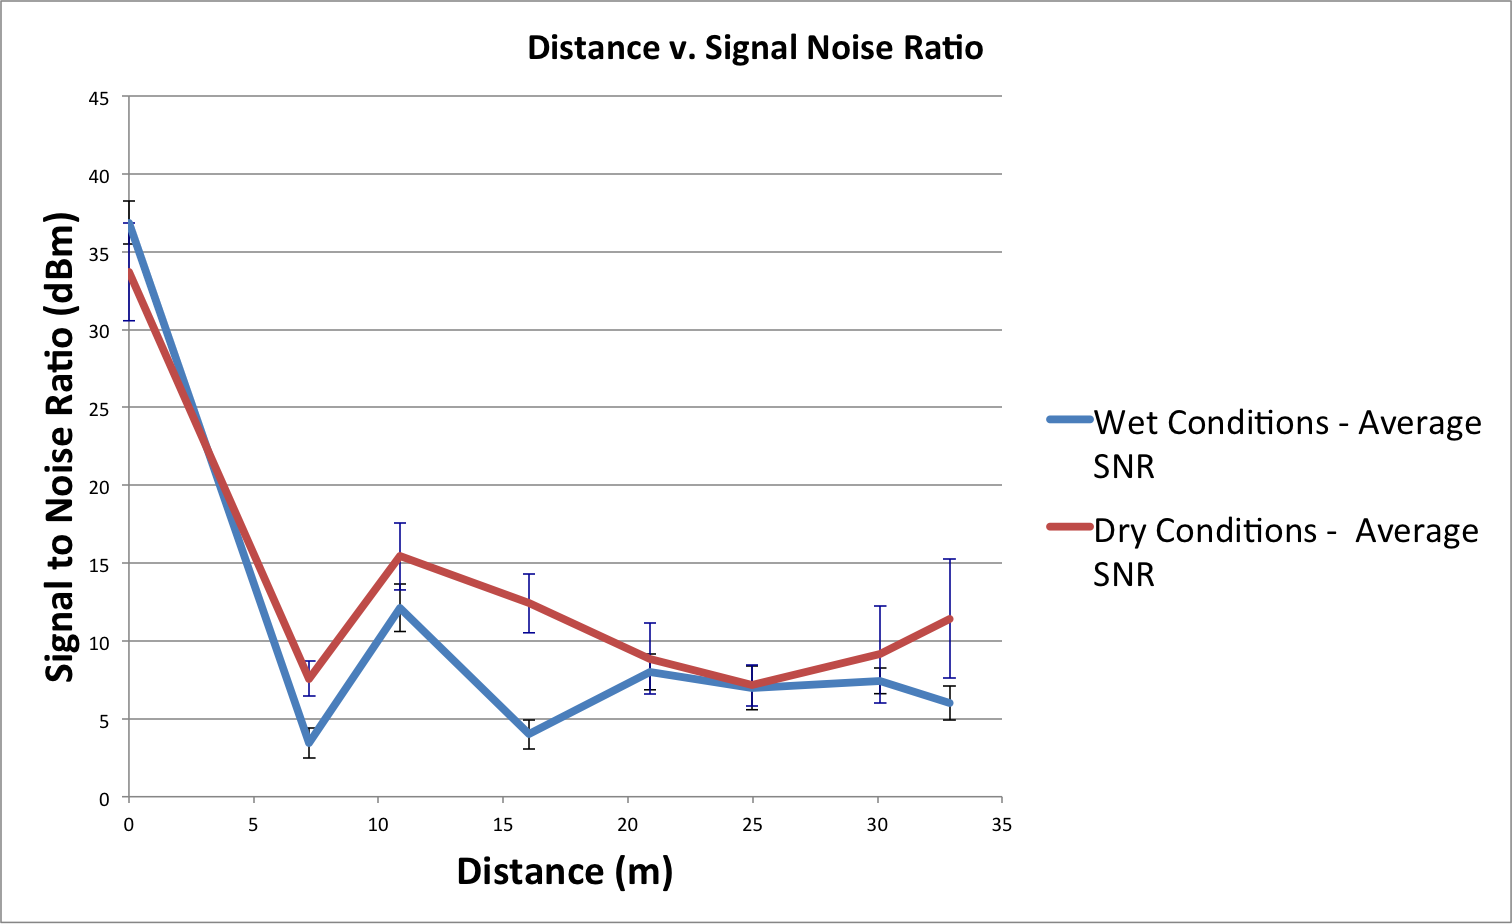
\includegraphics[width=\textwidth]{Chap3/figures/dg_snr.png}
%   \caption{Malaysian Rainforest}
%  \label{malaysiasnr}
% \end{subfigure}
\caption{Signal-to-Noise Ratio for Wi-Fi}
\label{fig:test}
\end{figure}
						
			Figure \ref{fig:test} shows that the maximum distance to receive a signal is approximately the same in Malaysia as it is in the UK.  There are more signal drops but this seems to be due to denser foliage blocking the line of sight. However, it does suggest that the humid environment of the rainforest does not have a significant impact on the received signal. It is clear that the denser rainforest does impact the signal-to-noise ratio in a much shorter distance from the base station but a link is still made, allowing for a successful transmission of data.
			
Poor Wi-Fi performance led us to research alternative methods to increase the range without impacting the environment the network is to be deployed in. We considered using intermediate nodes, not attached to cameras, to account for the lack of range but, because some cameras can be up to 1km apart, we would need more than 30 nodes to create a connection between two locations.
			
We also researched wireless technologies that are more common in sensor networks. This does mean that the data rate is not as high as Wi-Fi and error correction in packet streams is not always as robust, but it is more suited to sensor networks, using less power and providing longer range.
			
Finally, we considered using the researchers or animals at Danau Girang, as `data mules', creating temporary links between nodes while they are in the forest. However, the trip to Danau Girang yielded the information that researchers generally do not cover those distances in the forest and data delivery would be sporadic.

\subsection{DigiMesh}\label{tech:range:digimesh}
		Due to the poor range results of Wi-Fi, we created a second prototype of the network, using DigiMesh. DigiMesh is a proprietary wireless protocol, based on the 802.15.4 standard and designed for devices with limited power. Using the same frequency as Wi-Fi, DigiMesh has been reported to provide 7km of range, with a data rate of 250kbps.
		
In our prototype implementation, we are using Waspmote sensor boards \cite{waspmote}, a general purpose node that is capable of transmitting through various communication mediums. Our Waspmotes are provided with DigiMesh modules and a 2GB SD card to store sensed data.
		
When testing the range of the Waspmotes, we followed a similar method to that which is outlined in Section \ref{tech:wifi}. One board is in a fixed location and running a C++ application to poll for nodes in the network. Once a node is found it sends a message to the node every 10 seconds. The second board is set to scan the network and receive packets as soon as a base node is found; this node is then moved to different locations.
			
The receiving node prints out variables related to the received packet, such as: Received Signal Strength Indicator (RSSI), source MAC address and packet ID. However, not all packets are received so the RSSI can display 0 if there are errors in reading or if packet collision occurs. We found this to affect the results and have just used the two nodes to identify the maximum distance they can be apart, while maintaining a stable connection.
					
Initial experiments were run in a moderately vegetated area in the UK which yielded 497m of range. Limitations with buildings preventing us from testing any further but the signal strength still proved to be strong.
			
The initial results for the range tests were positive and DigiMesh does seem to be a viable solution to account for the lack of range when using Wi-Fi. As the frequency is the same as 802.11g, thus licensing it for worldwide use, we expected similar results in Danau Girang.
						
Experiments were run in 2 areas of the rainforest around Danau Girang and the results yielded were not the same as we experienced in the UK; the thick vegetation had a significant impact on the range, reducing it by almost 50\%.
			
In more open areas of the rainforest, we achieved 199m on average, more dense regions of the forest reduced this to 102m on average. While these results are not as high as we achieved in the UK, they are still suitable to use DigiMesh in the deployment of a WSN. The low range could be because we were using low-gain antennas and little configuration had been made on the DigiMesh radio.

\subsection{Adapting and Optimising for Harsh Environments}
	All of the hardware that we used for experiments had their components exposed, as shown in Figure \ref{tech:fig:nodes} and would have become compromised if moisture came in contact with them. To protect them from this, we used waterproof cases with a protective foam inside, known as Pelican cases, to keep the nodes watertight, but still allowing airflow to displace the heat generated, shown in Figure \ref{fig:tech:pelican}.
	External antenna can be fed through the lip of the case, using thin cable, ensuring that the range of the transmissions is not affected by the case. 

			\begin{figure}[H]
			\centering
			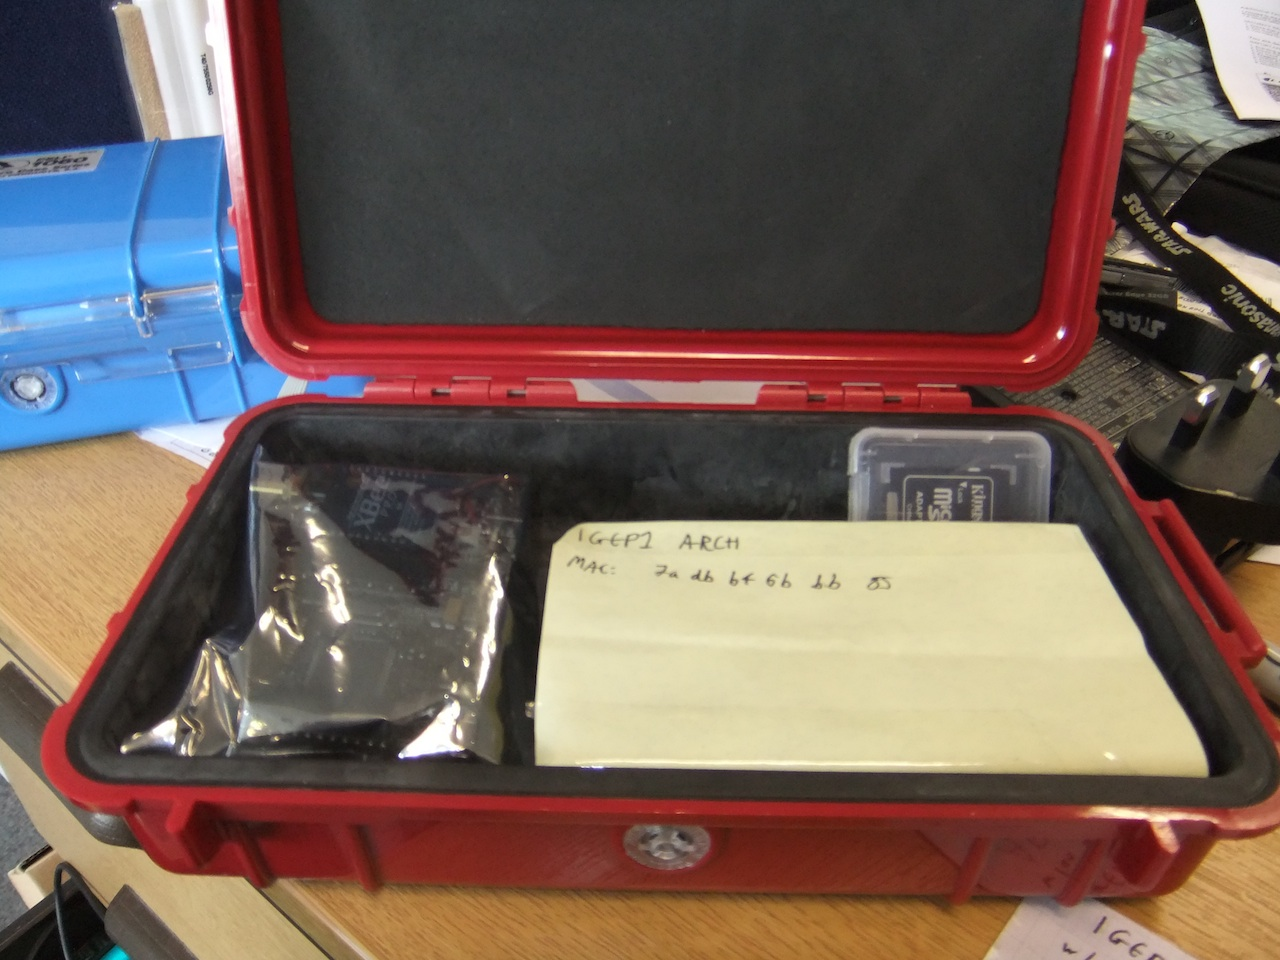
\includegraphics[width=\textwidth]{Chap3/figures/pelican}
			\caption{Pelican Waterproof Case}
			\label{fig:tech:pelican}
			\end{figure}

	After experiencing poor range results, we considered running antennae up through the trees to the canopy so there would have been no foliage to block signals and the humidity would have been lower. However, this was not possible because of conservation issues and the fact that animals could easily damage the antenna wire.

	Typically, WSNs in urban areas can use mains power and more remote networks utilise solar, or other renewable energy sources. In an area of dense foliage and high canopy cover, solar power is not a viable energy source. While DigiMesh has a lower transmission rate than Wi-Fi, its power requirements are lower, which maximises network lifetime for WSNs that do not have access to constant power or a renewable energy source.

\section{Software}\label{tech:sw}
	In this section, we explain the image processing software we developed for the real time processing of images within the network, as well as the retrospective processing of images that have been taken during previous deployments.

	\subsection{Triton} \label{tech:sf:triton}
		Triton is a C++ program that makes use of the Open Computer Vision (OpenCV) library \cite{opencv_library} for performing popular image processing functions \cite{triton}. Triton takes in a set of images, combines them and builds a Gaussian background model \cite{Zivkovic2004}, a common background subtraction method commonly available in many computer vision packages. Using this model, the foreground is extracted from the image and this is scanned for objects. If an object is found, it is extracted to a new image and saved as a black and white template. This minimises the memory each template takes up but can still be used to assist with future classifications. An object identified from a set of images means that the set is then marked as interesting, i.e. it is believed to contain something. If no object is extracted, it is marked as empty. The template extracted can the be classified by a human and, in the case of our motivating scenario, those classified templates can be used with newly sensed images to determine a match and allow for classifications down to the species level.
		
		Primarily, we developed this tool to detect the large number of empty images captured around Danau Girang, due to trees falling, movement of the Sun, fast animals or dirt on the lens. However, Triton proved to be quite effective when finding images of interest and it was modified to be used with our sensors. In this section, we explain how Triton was tested and compared with human observations. To ensure a valid comparison, we also compared both results to a random classifier.
	
		During a typical three month deployment along the Kinabatangan River more than 40,000 images can be taken. A large proportion of these images can be classed as \textit{false triggers}; occurring when a camera is triggered by the motion detector but there is no object of interest. These can be caused by changes in the light, falling trees or animals moving too fast to remain in the shot in the delay between the motion detector triggering and the camera capturing an image.
		
		We organised the images collected by the original camera that captured them and separating them into sets of three, because that is the number of images that the cameras were configured to take at each trigger. From this, we built a Gaussian background model \cite{Zivkovic2004} for each set and used the resulting model to detect objects in the foreground, classifying the detected foreground as the Region Of Interest (ROI), and extracting it.
	
		Figure \ref{tech:reconyx} shows a sequence of images taken by a Reconyx HC500 camera. The dynamic background and light levels make it very difficult to extract an object of interest. A background model is built from these images, which contains everything that is believed to be in the background. In this case, it should be the ground, the trees and the visible sky. The background is then subtracted from the image, leaving the foreground, and ROIs, larger than a user-defined threshold, are identified. The largest ROI is then extracted from the image and saved separately, shown in Figured \ref{tech:reconyx:processed}.

\begin{figure}[ht!]
\centering
\begin{subfigure}[b]{0.5\textwidth}
  \centering
  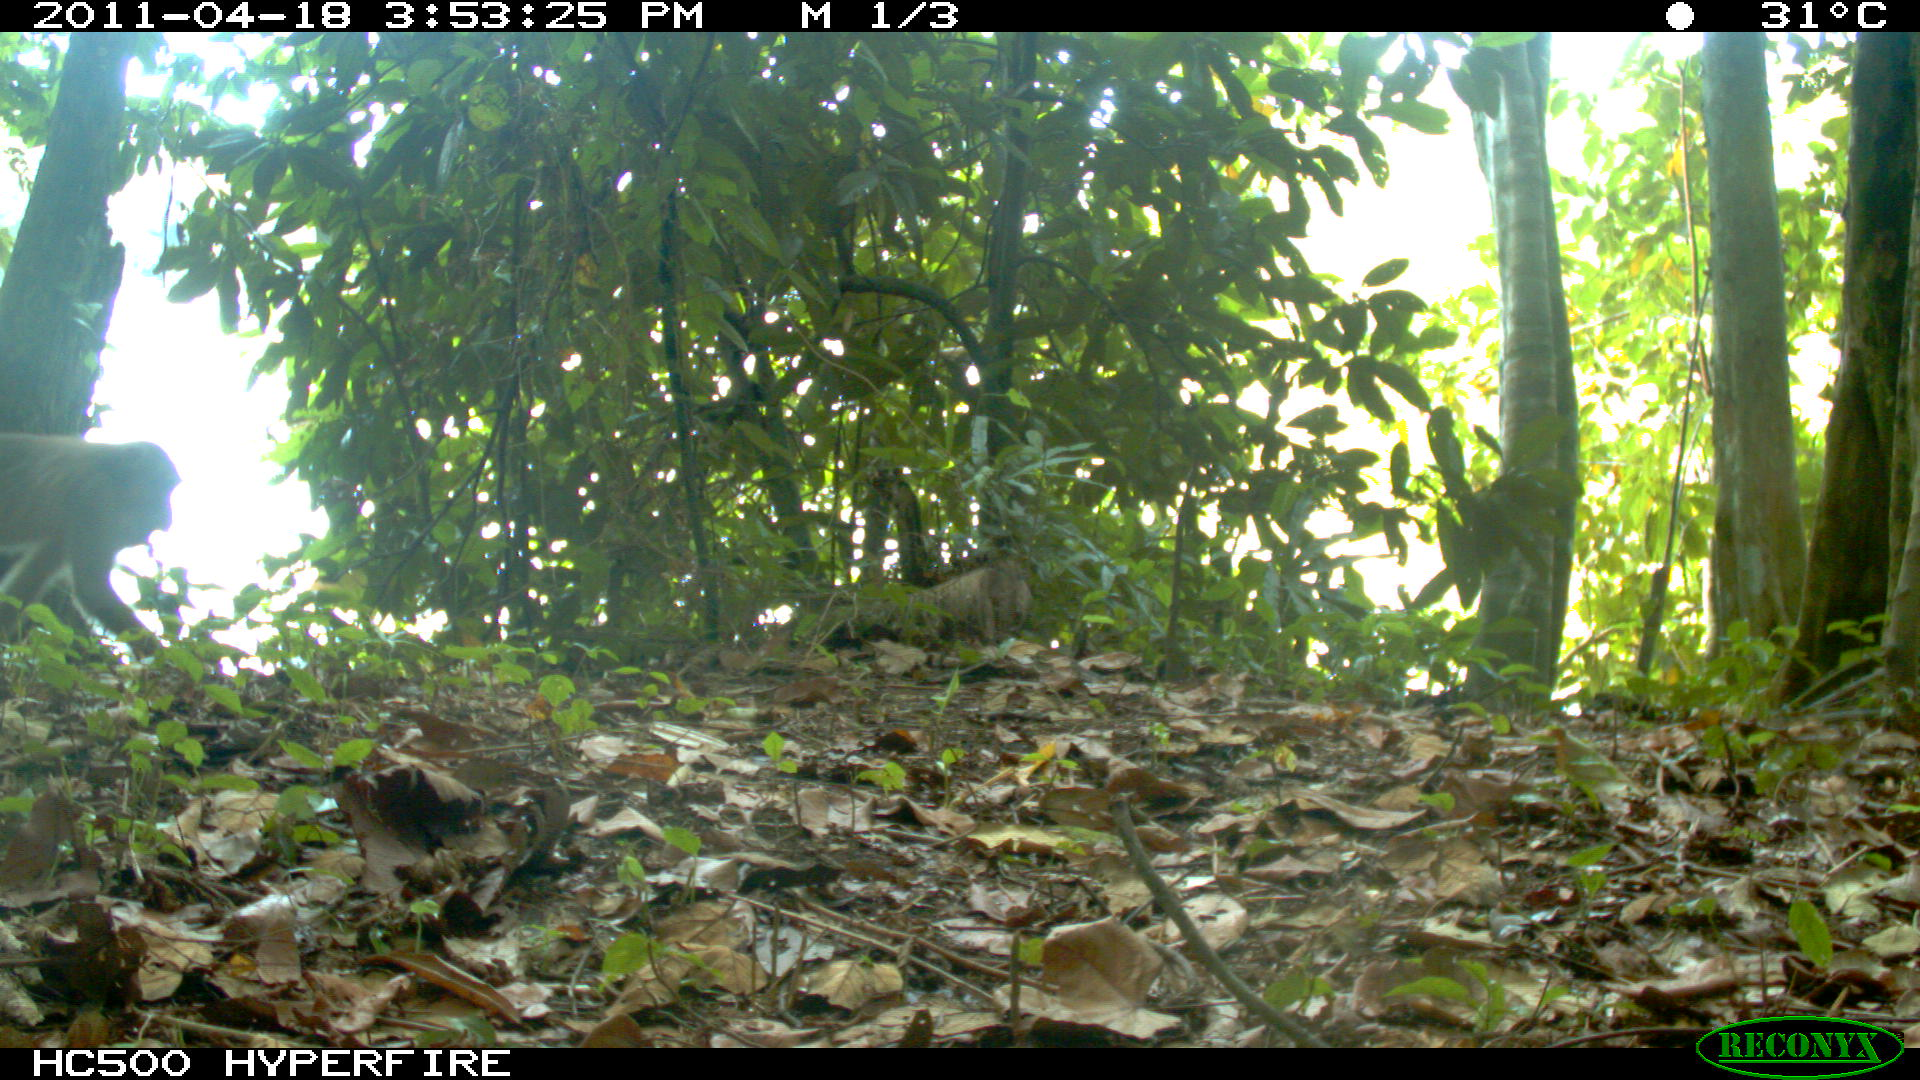
\includegraphics[width=\textwidth]{Chap3/figures/IMG_0568}
  \caption{Image 1 of 3}
\end{subfigure}%
\begin{subfigure}[b]{0.5\textwidth}
  \centering
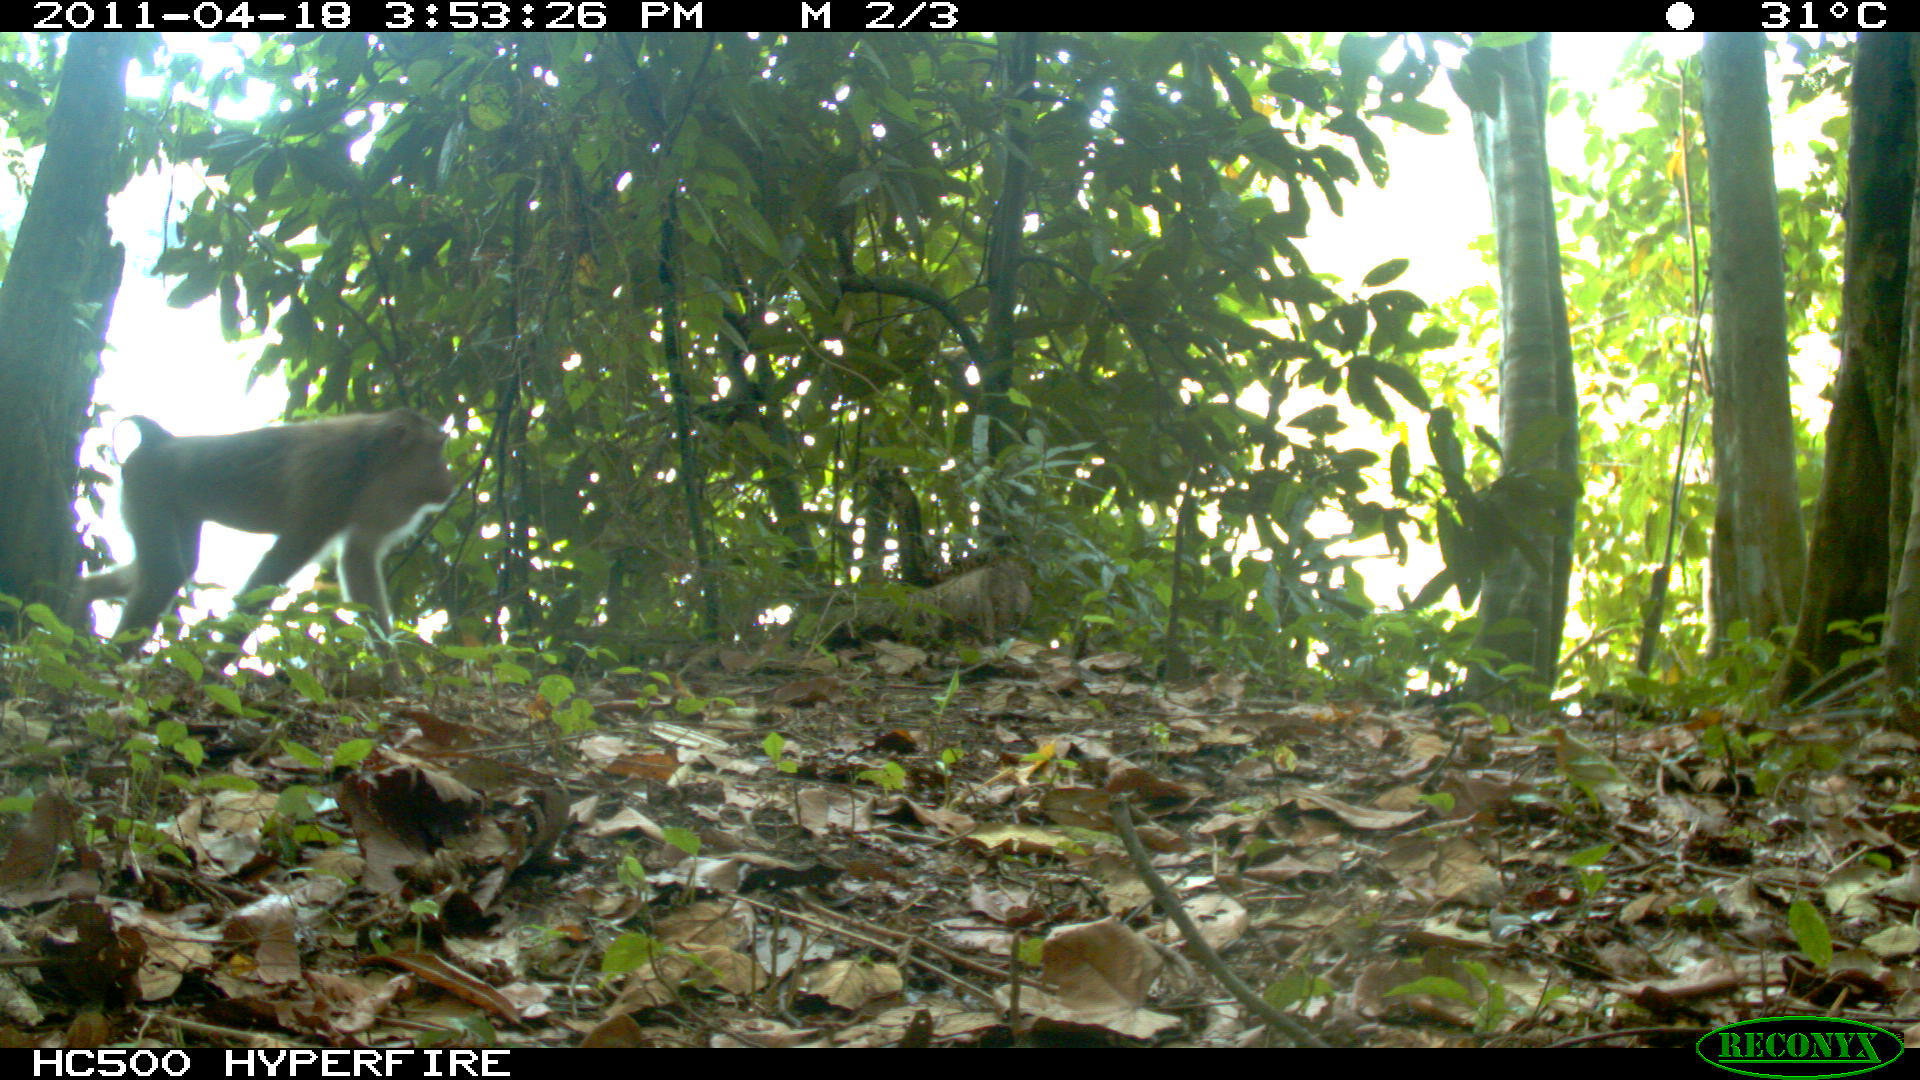
\includegraphics[width=\textwidth]{Chap3/figures/IMG_0569}
  \caption{Image 2 of 3}
\end{subfigure}
\begin{subfigure}[b]{0.5\textwidth}
  \centering
 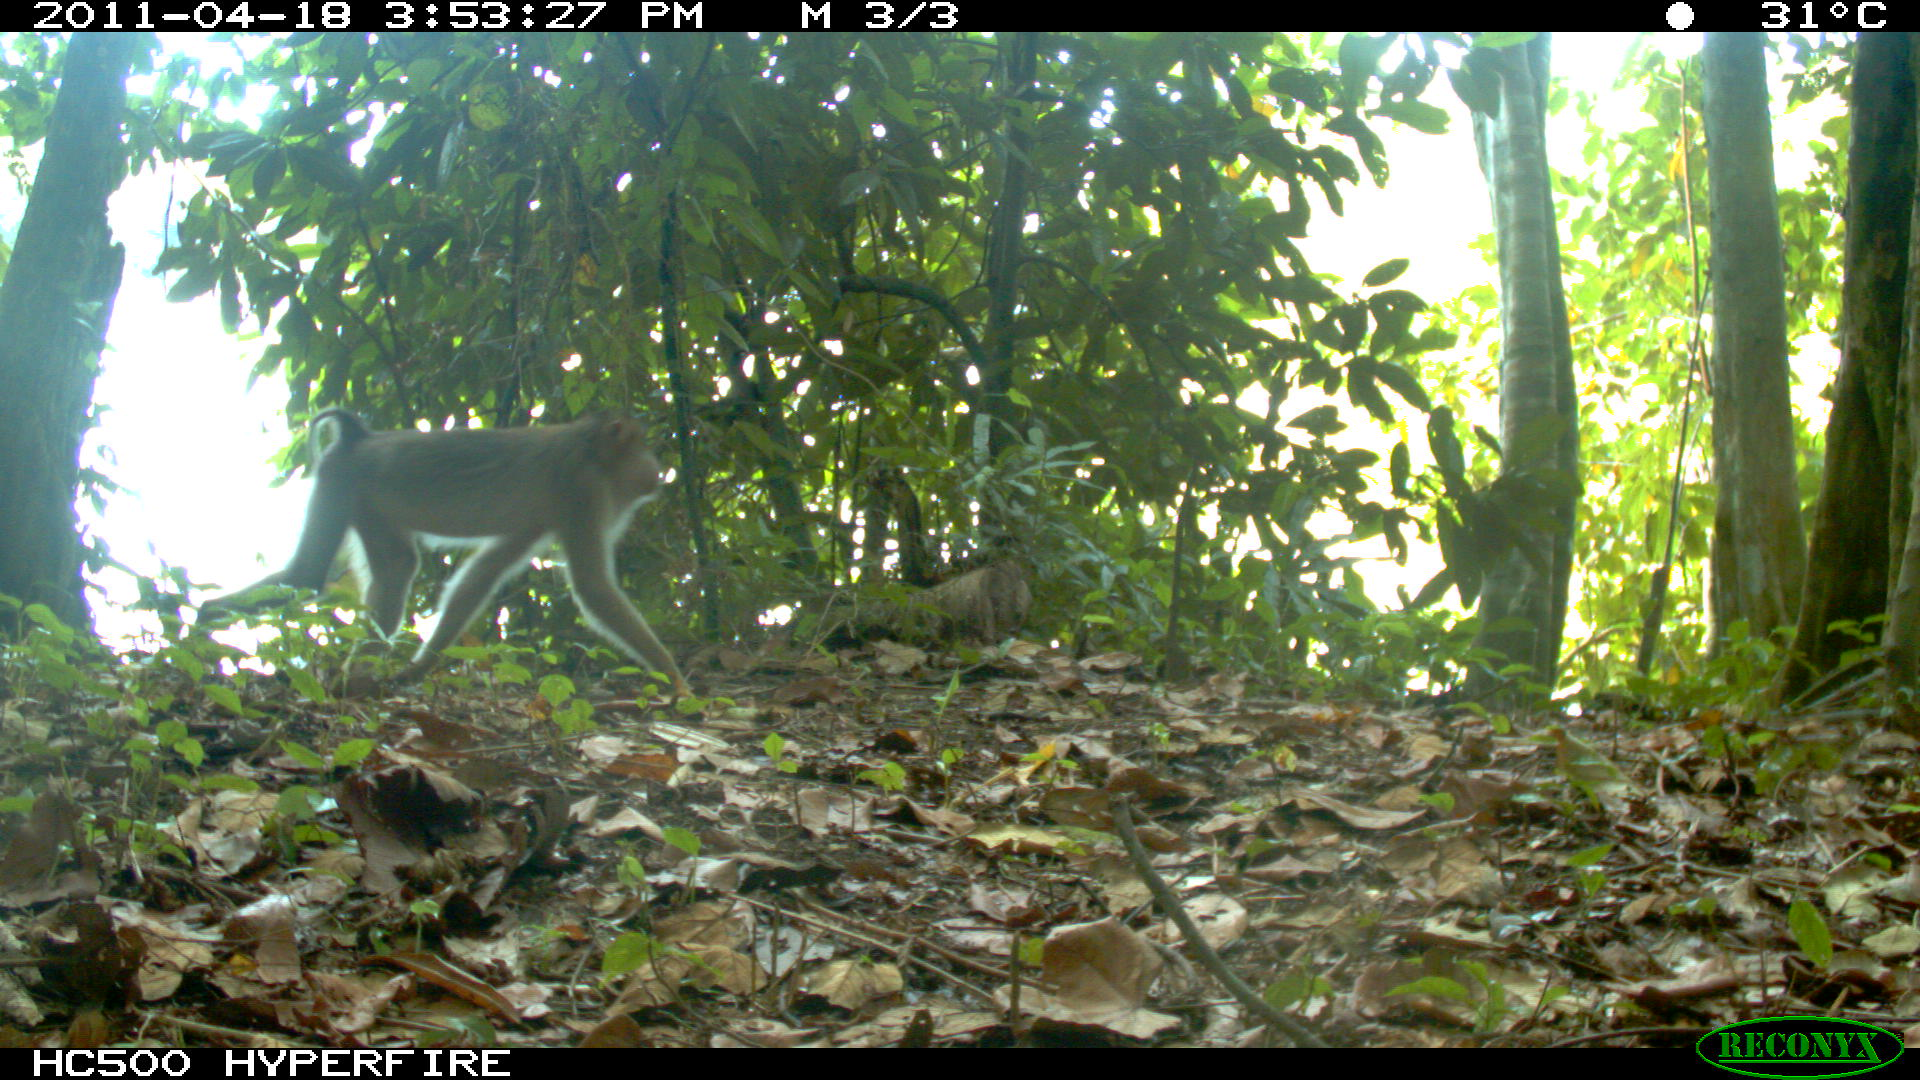
\includegraphics[width=\textwidth]{Chap3/figures/IMG_0570}
  \caption{Image 3 of 3}
\end{subfigure}
\caption{Sequence of 3 Images Captured on a Reconyx Trigger}
\label{tech:reconyx}
\end{figure}

			\begin{figure}[h]
			\centering
			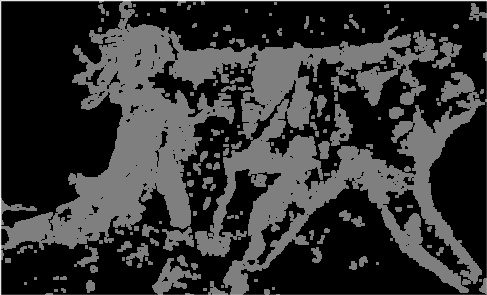
\includegraphics[width=\textwidth]{Chap3/figures/PROC_IMG_0568}
			\caption{Resulting Processed Image from Original Set of 3}
			\label{tech:reconyx:processed}
			\end{figure}
	
		From our visit to Danau Girang in 2011, we collected images from two different three month deployments, with the same cameras placed in different sites around Danau Girang for each deployment, giving us just over 70,000 images to test our approach. The images are sorted by the camera location and the date of collection. We process every 3 images as one set, building a background model of all three images.
		
		We manually processed all of the images initially, marking images that are empty as false triggers. We then processed the images, using our application, and a resulting processed image is created from every set of 3 images. If nothing is detected in a set then no image is created and that set is logged as empty. 
		
		There are four classifications that can be made with images sets:
		\begin{description}
			\item True positive: An ROI is extracted that contains the animal in the set.
			\item False positive: An ROI is extracted that contains nothing of interest.
			\item True negative: A camera is triggered with nothing of interest in the image and no ROI is extracted.
			\item False negative: An image containing an animal has no ROI extracted.
		\end{description}
		
		The processed images are then compared with our manual findings. The accuracy of our application is calculated by the following equations:
		
		%\begin{equation}Accuracy = (T_{p} + T_{n})/Total Sets\end{equation}
		\begin{equation}\label{ac:tp}  Accuracy_{tp} = (Ex_{tp} / Ac_{tp}) * 100 \end{equation}

		\begin{equation}\label{ac:tn} Accuracy_{tn} = (Ex_{tn} / Ac_{tn}) * 100 \end{equation}	
		
			Where Ex$_{tp}$  is the number of true positive sets extracted, Ac$_{tn}$  is the actual number of true positive sets, Ex$_{tn}$ is the number of true negatives extracted and Ac$_{tn}$ is the actual number of true negative sets.
		
		Table \ref{table:processing} shows experiments run on images from a randomly selected camera deployed in Danau Girang, testing on 300 sets of 3 images. These images were manually processed and classified as interesting or empty, of the 300, 94 sets were identified as interesting. Using Triton, 77 of those interesting sets (true positives) were extracted, with another 17 false positives extracted. 201 true negatives were correctly identified and a further 5 were identified as false negatives. As Triton processed these sets, we tested the time it took to complete a set of images on a Pandaboard and we found the mean time to be 43 seconds. 
		
		Out of the 94 interesting sets, 77 were identified correctly, giving an accuracy of 82\% for finding true positives (using Equation \ref{ac:tp}. Furthermore, of 206 empty sets, 201 were found, which gives a 98\% accuracy at correctly identifying true negatives, using Equation \ref{ac:tn}.
	
		These preliminary results show that our method is effective at detecting images of interest (True Positives) and it appears that misclassifications (False Positives) primarily came from black and white images taken at night, images where minimal movement of the animal has caused a trigger and images where an animal has caused a trigger but it has been too fast moving to be in the second two images.
		
		After a longer deployment, we would be able to build up a more substantial background model to account for some of the animals being less dynamic in images and we expect this to decrease our error rate thus reducing the number of false negatives, although this is something that is yet to be implemented.
		
		\begin{footnotesize}
		\begin{table*}
		\centering
			\hfill{}
			\begin{tabular}{|l|l|c|c|c|c|}
				\hline
					True Positive & True Negative & False Positive  & False Negative & Total Image Sets \\
				\hline
					77 & 201 & 5 & 17 & 300 \\
				\hline
			\end{tabular}
			\hfill{}
			\caption{Classification Results}
			\label{table:processing}
		\end{table*}
		\end{footnotesize}
		
		The results of Triton were compared to a random classifier, implemented in Python, that ran through a directory of images and generated a random number for each file. If the generated number was less than 0.25, then it was marked as true positive, between 0.25 and 0.49 marked it as false positive, between 0.5 and 0.74 was a true negative and between 0.75 and 1 was a false negative. Table \ref{table:random} shows the outcome, with 72 \textit{true positives} extracted, resulting in an accuracy of 80\% (using Equation \ref{ac:tp}. 73.3 \textit{true negatives} from a total of 206 were found, giving an accuracy of 36\% (using Equation \ref{ac:tn}). Although this set does not compare to the number of images collected in a six month deployment, human classification is a time consuming process and to have 900 classifications is complex. Although these could be crowdsourced, the reliability becomes questionable, in part due to the specialist nature of the images. This does show that our approach is quite close to the accuracy of a human when finding images of interest, but is able to do so in a fraction of the time, processing hundreds of images every minute. 
		
		Triton, coupled with a set of human eyes at the heart of the network, should be an effective approach for prioritising images through the network, even when a classification cannot be made through the use of local knowledge. More importantly, in an area where the environment is as dynamic as the Malaysian rainforest, 98\% accuracy for detecting true negative images can be crucial, if only for saving network bandwidth.
		
		\begin{footnotesize}
		\begin{table*}
		\centering
			\hfill{}
			\begin{tabular}{|l|l|c|c|c|c|}
				\hline
					True Positive & True Negative & False Positive  & False Negative & Total Image Sets \\
				\hline
					72 & 73.3 & 78.3 & 75.3 & 300 \\
				\hline
			\end{tabular}
			\hfill{}
			\caption{Random Classifier Results}
			\label{table:random}
		\end{table*}		
		\end{footnotesize}	
			%END OF INSERTION
%	
%	\subsection{ODACH}
	\subsubsection{Future Work}
		Triton is currently capable of processing a set of images and extracting the largest object of interest, if one is detected. The primary benefit of this is that it requires no training initially and works, with fairly good accuracy, from the time of deployment. However, functionality can be extended by storing the extracted images and associating it with the actual content, i.e. animal name, future extracted images can then be matched to the templates, within a threshold, to assist with classifications within the network. Currently, the templates are extracted, stored and associated with their contents once classified by a human, but Triton does not use these. If Triton detected an interesting image, it could then search a folder of templates and use OpenCV to compare the images and provide a cursory species classification based on the closest match. 
		
		Extracted images are stored in black and white and are only a few kilobytes in size, this will be useful as we expect that a large number of templates would be required in order to accurately identify an object of interest. For example, in our motivating scenario, an animal could be any distance from the camera, its legs could be in different positions or its angle it faces towards the camera could be different, giving many possible images. This process could be optimised by only matching regions between extracted images, such as the head or body, but this would require further experimentation.


\section{Conclusion}\label{tech:conc}
	In this chapter, we have shown the current hardware choices available for more computationally capable sensors and detailed our experimental results on how rainforest environments impact wireless transmissions. Although wireless technologies such as Wi-Fi provide a high data rate, their range is limited and not suitable for sparsely located nodes covering a large area; especially in a humid environment. Commercial Wi-Fi solutions are becoming more widespread in open, public places, such as: shopping malls, airports and universities, but these places allow for multiple routers, constant power supply and a greater range as routers are placed as high as possible to maximise coverage.
	Newer wireless technologies, designed for long-range communication in sensor networks, are becoming increasingly more viable and, while they do have lower data rates and less robust protocols, they are more suitable for a resource constrained WSN that requires minimal power draw when transmitting. 
	Using general-purpose hardware also means that there is no protection against water, humidity and animal or human intervention. We adapted existing waterproof cases to suit our needs and preliminary short term deployments showed that they are able to prevent moisture from entering the case.
	% Testing existing images on our software, Triton,  yielded positive results (97\%) for detecting empty images and also experienced success with finding images that had interesting content, resulting in 82\% accuracy.
	We have also developed an image processing application, Triton, that attempts to extract an object from a set of images that it believes to be the subject. Image sets that do not have any subject are classed as empty and should have no object extracted while those with a subject are interesting and should have an object extracted. Testing Triton on existing images at DGFC yielded 98\% accuracy for detecting empty image sets and an 82\% accuracy for finding interesting sets. A key feature of Triton is that it is not calibrated for a particular background or environment, so these results are especially promising.
	 
